\chapter{Estado del Arte}
\thispagestyle{empty}

En el campo del aprendizaje automático, el tema de la estimación de la distancia en fotografías faciales ha ganado recientemente mucha atención. La Figura \ref{fig16} muestra la tendencia ascendente de publicaciones que hacen referencia a la SCD. El número alcanza 441 artículos desde 1992 indexados en la base de datos Scopus \footnote{Las búsquedas se pueden consultar en el \hyperref[scopus]{Apéndice}.}.

\begin{figure}[H]
	\centering
	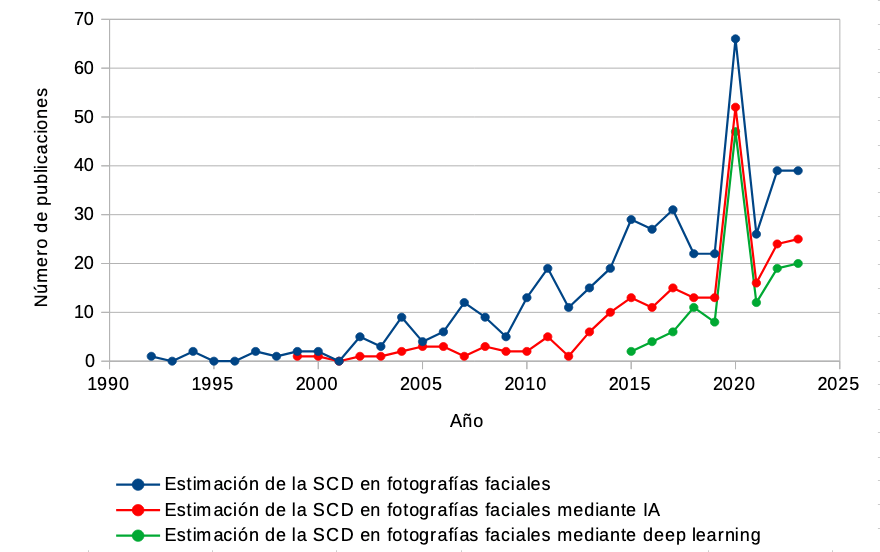
\includegraphics[scale=0.8]{imagenes/cap3/grafica_scopus6.png}
	\caption[Número de publicaciones sobre la estimación de la SCD.]{Número de publicaciones, en Scopus, relacionadas con la estimación de la distancia en fotografías faciales en función del año de publicación.}
	\label{fig16}
\end{figure}

El número de publicaciones relacionadas con este tema, ha ido en aumento a lo largo del tiempo, alcanzando un mayor número de publicaciones en 2020. En particular, a partir de 2015, se empezaron a aplicar técnicas de aprendizaje profundo. Este cambio se debe a los avances tecnológicos que han permitido la implementación de nuevas estrategias y conocimientos.

Sin embargo, a pesar de existir 411 publicaciones relacionadas con la SCD, son escasas las investigaciones que tratan el problema específico que aborda este trabajo. La mayoría de ellas se enfocan en el desarrollo de técnicas para inferir la profundidad de los objetos capturados en la imagen, analizando meticulosamente la disposición y las relaciones entre los elementos de la escena fotográfica. Estos enfoques buscan identificar patrones visuales que revelen información sobre la distancia relativa de los objetos o individuos a la cámara, sin considerar necesariamente la relación directa con esta última.


\section{Estimación métrica de la SCD}

Uno de los primeros métodos utilizados para abordar la estimación métrica de la SCD a partir de una imagen facial, fue propuesto por Flores et al. \cite{28}, quienes proponen utilizar un conjunto de puntos de referencia faciales para calcular la distancia y la posición respecto a la cámara, en un rango que va desde los 10 cm hasta los 3 m.
Este método consiste en tomar una imagen 2D de una cara desconocida, identificar sus puntos de referencia faciales y compararlos con los puntos obtenidos de modelos faciales 3D conocidos. Luego, empleando el algoritmo EPnP \cite{29}, se determina la distancia entre la cámara y el sujeto. Esta técnica asume que los puntos de referencia no varían significativamente entre individuos, sino que tienden a agruparse en \textit{clusters}.

Sin embargo, este primer enfoque presenta algunas limitaciones, como la dependencia de conjuntos de datos en 3D (los cuales no siempre están disponibles), la mezcla de diferentes distancias focales en un mismo conjunto de datos y la necesidad de reconocimiento manual de los puntos de referencia faciales.

Posteriormente, Burgos-Artizzu et al. \cite{30} introducen un método innovador que elimina la necesidad de anotación manual de los puntos de referencia de la imagen. En su lugar, estos puntos se estiman automáticamente mediante un enfoque de regresión conocido como \textit{Robust Cascaded Pose Regression} (RCPR) \cite{53}. Una vez que se han identificado los puntos de referencia faciales, se emplea un modelo automático de regresión para predecir la distancia entre la cámara y el sujeto en función de la posición relativa de estos puntos. Este regresor fue entrenado utilizando el conjunto de datos Caltech Multi-Distance Portraits (CMDP) \cite{54}, que consta de 53 retratos individuales tomados desde 7 distancias diferentes, que van desde 60 cm hasta 480 cm. Todos estos retratos están anotados manualmente con 55 marcas faciales.

Este método, sigue teniendo algunas limitaciones como el recorte de las imágenes (pérdida de resolución) o la única vista frontal.

Además de los métodos previamente citados, se han desarrollado otras técnicas para estimar la SCD basadas en características anatómicas como el tamaño facial \cite{32}, la separación entre los ojos \cite{33}, o una combinación de ambos factores \cite{34}.

\subsection{Estimación basada en características anatómicas}

En 2017, Stephan et al. \cite{20} desarrollaron un método para la estimación de la SCD en imágenes faciales llamado PerspectiveX. Este método fue diseñado para mejorar el proceso de superposición craneofacial y se basa en la localización de una característica anatómica específica, la longitud de la fisura palpebral, definida por dos puntos de referencia fácilmente identificables. 

Esta elección se justifica por varios aspectos: su clara visibilidad frontal, incluso cuando la cabeza experimenta un ligero giro hacia el lado más cercano a la cámara; su definición precisa, que garantiza una correcta medición; su mínima variabilidad, atribuible a restricciones evolutivas; su notable tamaño facial relativo, lo cual minimiza la probabilidad de errores en comparación con características más pequeñas, como el diámetro del iris; y su distribución normal, que contribuye a reducir el margen de error en las predicciones. Sin embargo, dado que la longitud real de la fisura palpebral puede no estar disponible, se recurre al promedio de un grupo demográfico homogéneo en términos de sexo y edad, ya que se sabe que esta medida varía mínimamente debido a restricciones evolutivas.

Junto con la longitud de la fisura palpebral, PerspectiveX requiere conocer el tipo de cámara, necesario para obtener las especificaciones de píxeles, así como la distancia focal de las lentes. Ambos datos pueden extraerse de las imágenes electrónicas mediante lectores EXIF disponibles en línea. Finalmente, la estimación del SCD se realiza mediante la siguiente fórmula:

\begin{equation}
	SCD = f (1+\frac{A}{x \cdot y})
\end{equation}

donde: $f$, es la distancia focal de las lentes (mm); $A$, es la longitud real de la fisura palpebral (mm); $x$, es la longitud de la fisura palpebral en la foto (píxeles); $y$, son las especificaciones del tamaño del píxel del receptor de imagen (mm).

A pesar de que PerspectiveX ofrece una estimación precisa de la SCD para una distancia focal conocida, también presenta ciertas limitaciones. Estas incluyen la necesidad de intervención manual para marcar los puntos de referencia faciales y la incapacidad para considerar las rotaciones de cabeza que superen los 30°. Además, se llevó a cabo un estudio para validar el algoritmo, utilizando fotografías tanto de vista frontal como de perfil, tomadas con cámaras DSLR y \textit{smartphones} \cite{70}. Si bien los resultados fueron satisfactorios para las fotografías obtenidas con cámaras DSLR, se observaron imprecisiones notables en las tomadas con \textit{smartphones}, tanto en la vista frontal como en la de perfil.

Posteriormente, en 2020, surge MediaPipe Iris \footnote{https://blog.research.google/2020/08/mediapipe-iris-real-time-iris-tracking.html}, un modelo de aprendizaje automático desarrollado por investigadores de Google. Este modelo tiene la capacidad de rastrear puntos de referencia como el iris, la pupila y los contornos del ojo en tiempo real, utilizando únicamente una cámara RGB estándar y sin necesidad de utilizar ningún hardware especializado. Mediante el seguimiento de los puntos de referencia del iris, este modelo puede determinar la distancia métrica entre el sujeto y la cámara.

El modelo se basa en el diámetro horizontal del iris del ojo humano, el cual se mantiene relativamente constante en un rango de 11.7±0.5 mm en una amplia población. Esta característica, combinada con argumentos geométricos simples, permite al modelo estimar la distancia SCD.

Sin embargo, es importante destacar que este modelo presenta ciertas condiciones y limitaciones. Es útil únicamente en situaciones donde existan datos EXIF disponibles, se capturen imágenes frontales donde el iris sea visible, y los individuos se encuentren a una distancia de menos de 2 metros de la posición de la cámara.

\subsection{Técnicas \textit{deep learning}}

A finales de 2022, Bermejo et al. \cite{14} presentan un novedoso método que estima la SCD directamente a partir de fotografías mediante el empleo de técnicas de aprendizaje profundo. La utilización de una arquitectura de redes neuronales profundas elimina una restricción crucial: la necesidad de detectar una característica anatómica específica para guiar el proceso de estimación. Esta capacidad permite que el método sea eficaz en la estimación de la SCD en cualquier posición de la cabeza, desde la frontal hasta el perfil lateral.

Este método se compone de cuatro modelos de aprendizaje profundo basados en la arquitectura VGG-16, cada uno asociado a una distancia focal específica: 27 mm, 35 mm, 55 mm y 85 mm, respectivamente. Para entrenar estos modelos, se empleó un conjunto de datos híbrido que incluye dos colecciones: una colección sintética de aproximadamente 150.000 imágenes generadas a partir de los modelos 3D disponibles en la base de datos Stirling ESRC 3D Face \footnote{Stirling ESRC 3D Face: https://pics.stir.ac.uk/ESRC/}; y una colección de fotografías digitales de 28 individuos tomadas a diversas distancias, desde 50 cm hasta 6 m, y en siete posiciones diferentes de la cabeza, desde el perfil izquierdo hasta el perfil derecho.

Este enfoque destacó por varias características clave, entre las cuales se incluye la utilización de pesos preentrenados en el conjunto de datos ImageNet \cite{97} como punto de partida para la inicialización de los modelos, acelerando así el proceso de entrenamiento. Además, se empleó el error absoluto medio de la distorsión facial relativa como medida principal de rendimiento, lo que contribuyó a mejorar la precisión en la estimación de distancias cortas, que suelen presentar una mayor distorsión.

Los resultados obtenidos por FacialSCDnet son prometedores. En la Sección \ref{fscdnet} analizaremos con más detalle las características de este médoto así como las limitaciones que justifican el desarrollo del presente TFG.